\chapter{Experimental setup}
\label{chapter:environment}

This chapter portrays the scope and the environment used for the presented experiments. More specifically, \Cref{section:scope} describes the scope and research design of this work. Section \ref{section:data} presents an overview of the training dataset from the \ac{ISIC} 2019 challenge, discuss its class distribution, and also outlines the dataset for the unknown class. \Cref{section:preprocessing} explains the preprocessing steps applied to the dataset samples before training. \Cref{section:augmentation} catalogues several augmentation techniques used further in some of the experiments, along with examples. \Cref{section:split} describes the dataset split process into train, validation and test sets. \Cref{section:hardware} provides a synopsis of the hardware resources used for the experiments. Finally, \Cref{section:software} presents the software stack used for training and testing models, along with arguments for the choices of the frameworks and tools used.

\section{Experimental Scope}
\label{section:scope}
    This work is concerned with the development of a multi-class dermoscopic image classifier for the diagnosis of different types of skin lesions. The classification problem will be addressed using \ac{CNN} models, focusing on the process of designing the classifier from a set of training examples and the process of evaluating the generalization performance of the classifier. \par
    
    To create an end-to-end \ac{CNN} classifier of skin lesions through deep neural networks, one of two approaches can be chosen. The first is to create a model from scratch, which implies designing its architecture, cross-validation a wide range of hyperparameters, choosing the weight initialization method and train it from the ground up. However, this approach is troublesome because it requires thorough reasoning for each of these tasks. In practice, this requires cross-validating a wide range of hyperparameters and network design related parameters, which can be time-consuming and computationally expensive. \par
    
    However, another approach is using transfer learning by leveraging the weights of pre-trained models. This is a good option when data is scarce, which is often the case for medical imaging-related classification tasks \cite{Ching2018}. Additionally, there is a wide range of pre-trained models to choose from, because of benchmark challenges such as the \ac{ILSVRC}. For the presented experiments, the choice towards which models to study is based on commonly used ones presented in the literature (see \Cref{section:skin_transfer_learning}), and in their availability through the \verb|tf.keras.applications|\footnote{\url{https://www.tensorflow.org/api_docs/python/tf/keras/applications}} framework. More specifically, VGG16, VGG19, ResNet50, ResNet101, ResNet152, InceptionV3, InceptionResNetV2, DenseNet121, DenseNet169, and DenseNet201. \par
    
    Furthermore, although EfficientNets are not available in the \verb|tf.keras.applications| framework, some of its variants will also be tested due to their remarkable performance on the ImageNet dataset (see \autoref{tables:pretrainedmodels}). Namely, the shallower and smaller variants such as the EfficientNetB0, the EfficientNetB1, and the EfficientNetB2. Even though there are bigger EfficientNet models, the hardware setup used (further described in Section \ref{section:hardware}) is not able to properly train models larger than EfficientNetB2. Therefore, it has been decided to left them out of this work. \par
    
    Moreover, the holdout method will be used to make assessments, in which a different set of data to the training set, called the validation set, is used so to obtain an unbiased evaluation of the model’s generalization performance. The validation set is required because if one uses the test set for this optimization then there is a high risk of optimistically biasing the model \cite{talbot}. Even though the holdout method has its downsides, the time requirements are much lower compared to techniques like k-fold cross-validation, which is appealing to speed up experiments. \par
    
    One important challenge in applying \ac{CNN} to medical imaging is the large amount of labeled data required in order to achieve a performance that surpasses the shallow neural networks. The contributes of the \ac{ISIC} have been relevant in providing an open-source public access archive of skin images. This publicly available archive has been used for teaching purposes and the development of automated skin lesion diagnosis systems \cite{isic2019}. At the same time, the challenges proposed annually around a specific dataset facilitate better comparisons between new and existing solutions by standardizing evaluation criteria. The difficulties in monitoring and comparing progress in the field are the result of several factors, among which stand out non-standardized evaluation metrics, the use of different datasets, and differences in how learning tasks are framed \cite{Brinker2018}. Therefore, this work will use the \ac{ISIC} 2019 challenge dataset which provides 25331 image samples distributed across the 8 categories. \par
    
    In \Cref{section:metrics}, several metrics were presented to assess the performance of a machine learning model. Even though there are multiple metrics that one could use for multi-class problems with unbalanced data, the \ac{ISIC} 2019 organizers argue that \ac{BMA} is a good metric to compare different approaches on highly unbalanced datasets, because it penalizes strategies that optimize accuracy by preferring predictions in favor of the most prevalent class \cite{humanvsisic2018}. Hence, it is beneficial to use the \ac{BMA} as the primary metric of comparison in the presented experiments. \par 
    
    Furthermore, metrics like accuracy still strongly appear in the literature and can be used to understand whether a model is underperforming on underrepresented classes of the test set. This can be done by looking at the discrepancy between the accuracy and \ac{BMA} scores on the test set, in which if the accuracy is superior to the \ac{BMA}, most likely, underrepresented classes are underperforming in comparison with overrepresented classes. Therefore, the accuracy score will also be used to compare results in some of the experiments. \par 

\section{Data Representation}
\label{section:data}
    
    \subsection{Description}
    The \ac{ISIC} 2019 challenge \cite{isic2019} provides a training dataset with 25331 samples distributed across 8 different categories that can be represented within a hierarchy shown in \autoref{fig:hierarchy}. Such categories are:
    \begin{itemize}
        \item Melanocytic nevus (NV): benign neoplasms (excessive growth of tissue) of melanocytes (cells in the skin that produce and contain melanin) that appear in different variations that can be quite different from each other from a dermatoscopic point of view \cite{ham10000};
                
        \item Melanoma (MEL): a malignant neoplasm that is created from melanocytes and may appear in different variants. Melanomas either penetrate beyond the epidermis into the dermis (invasive) or not (in situ). If found the in early stages, Melanoma can be cured by surgical excision (\textit{i.e.}, removing the tissue) \cite{ham10000};
        
        \item Dermatofibroma (DF): benign skin lesion caused by an agglomeration of cells within the deeper layers of the skin. It can be caused by an adverse reaction to an injury (\textit{e.g.}, bug bite or splinter) \cite{ham10000};
        
        \item Vascular lesion (VASC): Birthmarks or childhood abnormalities of the skin and underlying tissues. It is composed of a collection of samples from cherry angiomas, angiokeratomas, pyogenic granulomas, and hemorrhages \cite{ham10000};
        
        \item Benign keratosis (BK): Benign lesions which include samples of solar lentigo (patch of darkened skin), seborrheic keratosis (harmless skin growth), and lichen planus-like keratosis (inflammatory reaction arising from solar lentigo or seborrheic keratosis) \cite{isic2019};
        
        \item Basal cell carcinoma (BCC): the most common type of skin cancer \cite{Foundation2019} that rarely metastasizes but grows destructively if untreated. It may appear in different variants such as flat, nodular, pigmented or cystic \cite{ham10000};
        
        \item Squamous cell carcinoma (SCC): the second most common form of skin cancer \cite{Foundation2019}, characterized by abnormal, accelerated growth of squamous cells. When caught early, most SCCs are curable \cite{Foundation2019};
        
        \item Actinic keratosis (AK): also called solar keratosis, it is a kind of abnormal skin cell development as a consequence of genetic code damage. It is considered to be an early form of invasive squamous cell carcinoma \cite{ham10000}.
    \end{itemize}
    
    \begin{figure}
      \centering
      \includegraphics[width=0.9\textwidth]{figs/skin_lesions_hierarchy.png}
      \caption[Hierarchical organization of skin lesions.]{Hierarchical organization of skin lesions. Taken from Barata \textit{et al.} \cite{Barata2020}.}
      \label{fig:hierarchy}
    \end{figure}
    
    This dataset is an agglomerate of samples from the HAM10000 \cite{ham10000}, BCN\_20000 \cite{bcn_20000}, and MSK \cite{msk}, all of which are labeled datasets of skin lesions. The \ac{HAM10000} dataset is an effort to boost research on the automated diagnosis of dermatoscopic images that focuses on the quality and reliability of a large volume of data. Images from \ac{HAM10000} belong to different sources and go through a pipeline to clean data. All of the samples are manually reviewed by dermatology professionals and non-dermatoscopic images or unreliable diagnoses are filtered out. Finally, all of the samples have the same resolution of 600x450 pixels centered around the lesion (see filtering process in \autoref{fig:ham10000}). The quality and volume of the data provided by this dataset is remarkably good and allows deep learning researchers to focus on developing reliable models rather than focus on extensive pre-processing methods before training. \par
    
    The \ac{HAM10000} had already been used in task 3 of the \ac{ISIC} 2018 challenge. The literature suggests that the top-scoring approaches of the \ac{ISIC} 2018 surpassed expert dermatologists \cite{humanvsisic2018}. However, as Tschandl \textit{et al.} pointed out, the algorithms performed worse on images from other dermoscopic data sources that were not present on the \ac{HAM10000} dataset \cite{humanvsisic2018}. This statement shows that the \ac{HAM10000} dataset alone does not provide enough samples that are representative of real-world scenarios. For example, real-world samples might not have the lesion centered or might be taken under different conditions (\textit{e.g.}, angle, luminosity, or contrast variations). \par
    
    \begin{figure}
      \centering
      \includegraphics[width=0.7\textwidth]{figs/ham10000.png}
      \caption[HAM10000 sample filtering process.]{\ac{HAM10000} sample filtering process. Taken from Tschandl \textit{et al.} \cite{ham10000}.}
      \label{fig:ham10000}
    \end{figure}
    
    As a countermeasure, the \ac{ISIC} committee added two more datasets to the \ac{ISIC} 2019 challenge, which would hopefully create enough variation and help \ac{ISIC} challenge metrics be representative of real-world scenarios. One of the new datasets is the BCN20000 \cite{bcn_20000}, which contains hard to diagnose images of size 1024x1024 captured between 2010 and 2016 by the Hospital Clinic in Barcelona. These images are often not correctly segmented, located in hard to diagnose locations such as nails or mucosa, and can even be hypopigmented, meaning that the overall color of the lesion is lighter than the skin tone. The resulting database includes 19424 manually revised dermoscopic images corresponding to 5583 skin lesions, meaning that some samples belong to the same lesion. \par
    
    Finally, the last new dataset is the MSK dataset, which contains images of multiple resolutions and multiple aspect ratios. The MSK is composed of multiple smaller datasets, namely:
    \begin{itemize}
        \item MSK-1 which contains images both from benign and malignant melanocytic lesions, but not taken with modern digital cameras. Almost all diagnoses were confirmed by histopathology reports, and the remainder consists of benign lesions confirmed by clinical follow-ups;
        \item MSK-2 composed of biopsy-confirmed melanocytic and non-melanocytic lesions. This dataset includes over 500 melanomas. Many images have polarized and contact variants;
        \item MSK-3 contains assorted images. Mostly composed of nevi and \ac{BCC} lesions. All diagnoses are confirmed through histopathology;
        \item MSK-4 composed of images belonging to patients with a personal history, clinical diagnosis, or differential diagnosis of melanoma. All diagnoses are confirmed through histopathology;
        \item MSK-5 composed of seborrheic keratoses obtained from patients during a clinical visit. These lesions were not biopsied and were determined to be seborrheic keratoses by agreement of three experts.
    \end{itemize}
    
    By looking at random samples from each of the eight classes of the \ac{ISIC} 2019 challenge dataset in \autoref{fig:samples}, one can observe that samples are quite different from each other. They often vary on aspect ratios, luminosity conditions, segmentation, cropping schemes and even the position of the lesion itself. Even within a particular class, an uninstructed person has a hard time pointing out common features, as some of the lesions can be hypopigmented or not be easily segmentable. Overall, the heterogeneity of this dataset aims to create a challenge that provides samples representative of real-world images of lesions, rather than filtered samples that are easy to diagnose \cite{bcn_20000}. \par
    
    \begin{figure}
      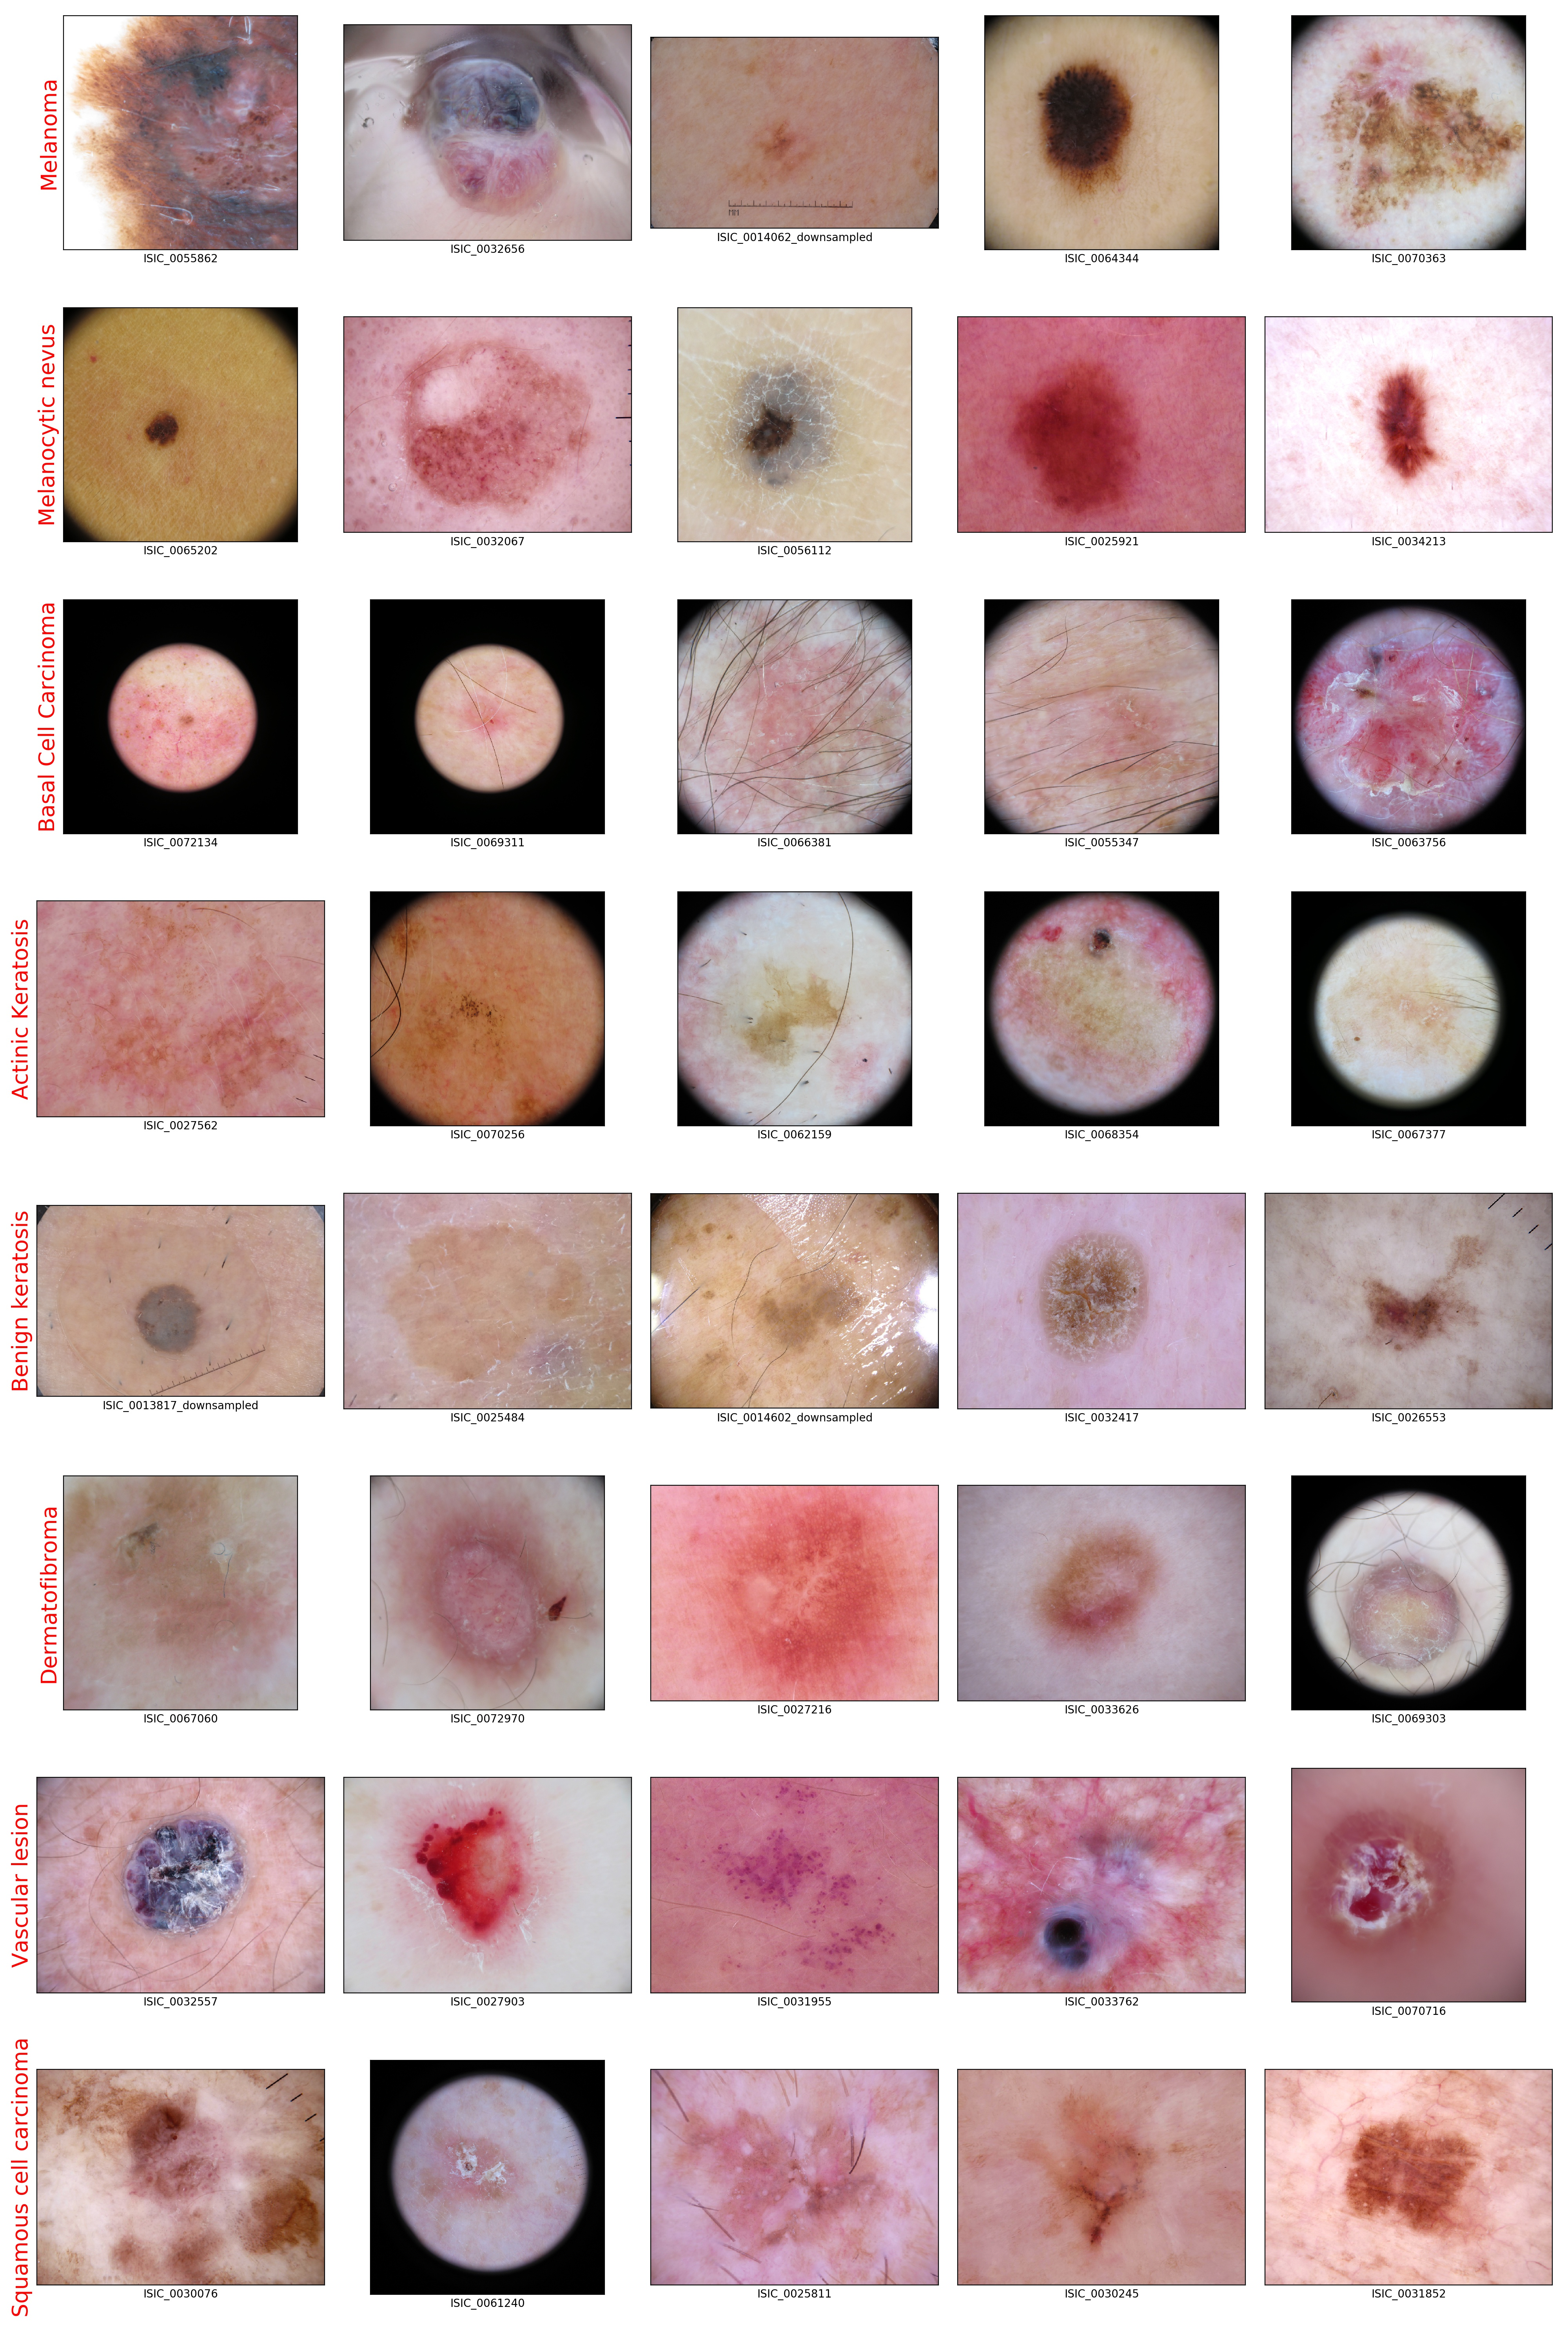
\includegraphics[width=\textwidth]{figs/samples_training_data.jpg}
      \caption{Samples from ISIC 2019 training data for the 8 known categories.}
      \label{fig:samples}
    \end{figure}
    
\subsection{Class Imbalance}
\label{subsection:imbalance}

    Note by looking into \autoref{fig:distribution} that the dataset provided is highly unbalanced with some classes like the melanocytic nevus (NV) representing almost half of the whole dataset, while a class like dermatofibroma representing less than 1\% of the dataset. \par
    
    \begin{figure}[h!]
      \includegraphics[width=\textwidth,keepaspectratio]{figs/training_data_distribution.jpg}
      \caption{Class distribution of \ac{ISIC} 2019 challenge training dataset.}
      \label{fig:distribution}
    \end{figure}

    To tackle this issue, a common method from other \ac{ISIC} 2019 approaches \cite{isic2019first}\cite{isic2019second}\cite{Wang}, is to use some kind of weighted loss function, like the weighted cross-entropy loss function. Following the comparisons done by Gessert \textit{et al.} \cite{gessert2018}, for the experiments, the weight $W_i$ of each class $i$ is defined as: \par

    \begin{equation}
        W_i=\frac{N}{C*n_i}
        \label{eq:class_weights}
    \end{equation}
    where $N$ denotes the total number of samples in the training set, $n_i$ is the number of samples for class $i$, and $C$ is the number of classes. \par

    This results in the weight distribution illustrated in \autoref{fig:weight_distribution}. One can observe that classes like dermatofibroma have a considerably higher weight than classes with more samples like melanocytic nevus. This means that the added loss from a misclassified sample of dermatofibroma will have a much bigger impact than a misclassified sample of nevi. Therefore, this method will avoid situations where the model tries to optimize weights towards overrepresented classes like nevi, rather than optimizing performance for each class individually. \par

    \begin{figure}[h!]
    \centering
      \includegraphics[width=0.7\textwidth,keepaspectratio]{figs/weight_distribution.pdf}
      \caption{Weights for each class of the weighted cross-entropy loss function in the \ac{ISIC} 2019 training dataset.}
      \label{fig:weight_distribution}
    \end{figure}

\subsection{Unknown Class}
\label{subsection:unknown}
    By looking at the sample distribution across the different classes in \autoref{fig:distribution} one can observe that no data is provided for the 9th class, namely, the "Unknown" class. This class is meant to represent none of the other classes, and it is meant to address some of the findings of Tschandl \textit{et al.} in which they noted that the accuracy from out-of-distribution test images was considerably worse than in-distribution test images \cite{humanvsisic2018}. \par
    
    The range of skin lesion diagnosis extends beyond the 8 classes represented in the \ac{ISIC} 2019 dataset (see \autoref{fig:distribution}). As such, when patients show a specific lesion to their dermatologist to diagnose, the lesion interpretation has to consider which type of lesion it represents, possibly not being part of the 8 categories represented in this dataset or possibly not representing a lesion at all. For example, it might be a scar, a bruise, or even normal skin. No data is provided for this class because it does not represent a specific category but rather an agglomerate of any skin fraction that is not part of the original training distribution. \par 
    
    Different strategies to deal with this unknown class will be experimented with in \Cref{chapter:experiments2}. However, for the analysis of the effectiveness of the experimented methods, an agglomerate of multiple samples was created to be categorized as unknown samples. Table \ref{tables:out_dist_dataset} shows the distribution of such samples. \par 
    
    \begin{table}[h]
        \centering
        \begin{tabular}{|l|r|r|}
            \hline
            \textbf{Lesion category}           & \multicolumn{1}{l|}{\textbf{Samples amount}} & \multicolumn{1}{l|}{\textbf{Source dataset}} \\ \hline
            Angiofibroma or fibrous papule     & 8                                            & \multirow{6}{*}{ISIC Archive}                \\ \cline{1-2}
            Scar                               & 4                                            &                                              \\ \cline{1-2}
            Angioma                            & 12                                           &                                              \\ \cline{1-2}
            Atypical melanocytic proliferation & 12                                           &                                              \\ \cline{1-2}
            Lentigo simplex                    & 22                                           &                                              \\ \cline{1-2}
            Lentigo NOS                        & 70                                           &                                              \\ \hline
        \end{tabular}
        \caption{Samples per category of skin lesion, for the "unknown" class.}
        \label{tables:out_dist_dataset}
    \end{table}
    
    All of the samples come from the \ac{ISIC} archive \cite{archive} and are left out from the \ac{ISIC} 2019 challenge because they do not belong to any of the original 8 classes. More specifically, they are part of the MSK dataset, which means that samples follow the same conditions to the other samples from the same dataset. This makes them quite similar to images from the \ac{ISIC} 2019 challenge training dataset for an uneducated observer (see \autoref{fig:unknown_samples}). As such, these samples will receive the same pre-processing as the samples from the original training dataset. \par
    
    \begin{figure}[h!]
        \centering
        \includegraphics[width=\textwidth]{figs/unknown_image_samples.pdf}
        \caption{Randomly chosen samples from the dataset created for the "unknown" class.}
        \label{fig:unknown_samples}
    \end{figure}


\section{Data Preprocessing}
\label{section:preprocessing}
    Each sample of the dataset undergoes several preprocessing steps, more specifically:
    
    \begin{enumerate}
        \item Most readily available pre-trained models are of network architectures whose input tensor is of square dimensions (\textit{e.g.}, $224 \times 224 \times 3$). Since the dataset's images are of distinct non-square dimensions, it is necessary to resize them to a square. However, naively resizing them to the network's input tensor dimensions without regard to each image's aspect ratio means that the input fed to the network is of varying distinct aspect ratios which does not constitute a good start. Therefore, the first step is to crop an arbitrarily-sized square of the center of the image (as per code snippet \ref{code:crop}) which will likely capture the skin lesion, as most images in the training dataset are centered around the lesion. \par
    
\begin{listing}[ht]
\begin{minted}{python}
def _crop(img):
    """
    Center crops the image with a squared aspect ratio (1:1).
    
    # Arguments
        img: PIL image.
    # Returns:
        the cropped image.
    """
    width, height = img.size
    # If already a square do nothing
    if width == height:
        return img

    length = min(width, height)

    # Define center crop box
    left = (width - length) // 2
    upper = (height - length) // 2
    right = left + length
    lower = upper + length

    box = (left, upper, right, lower)
    return img.crop(box)
\end{minted}
\caption{Function that crops a given image to a square crop of the center of the original image.}
\label{code:crop}
\end{listing}
    
    \item Even though different model architectures use different input tensor sizes, all images should be resized to the target network's input dimensions as soon as possible in the data pipeline. One can argue that by doing this process earlier will reduce the computational costs of applying this operation during the training process. Therefore, images are resized using nearest-neighbor interpolation before training the models.
    
% \begin{listing}[ht]
% \begin{minted}{python}
% def _resize(img, target_size):
%     """
%     Resizes an image to a target size using nearest neighbour interpolation
%     # Arguments:
%         img: PIL image.
%         target_size: tuple of (width, height) for the target image size
%     # Returns:
%     the resized image.
%     """
%     return img.resize(target_size, PIL.Image.NEAREST)
% \end{minted}
% \caption{Function that resizes a given image to the target dimensions.}
% \label{code:resize}
% \end{listing}

    \item Based on Gessert \textit{et al.} \cite{gessert2018}, each image is normalized by subtracting the channel-wise mean of the entire \ac{ISIC} 2019 training dataset, and then dividing it by its standard deviation (as in code snippet \ref{code:correct}). The channel-wise mean and standard deviation of the \ac{ISIC} 2019 training dataset was calculated beforehand. \par
    
        \begin{listing}[ht]
        \begin{minted}{python}
def preprocess_input(x):
    """
    Preprocesses a numpy array encoding a batch of images. 
    Each image is normalized by subtracting the mean and dividing by the standard deviation channel-wise.
    
    # Arguments
        x: a 3D numpy array consisting of RGB values within [0, 255].
    # Returns
        Preprocessed array.
    """
    if not issubclass(x.dtype.type, np.floating):
        x = x.astype(K.floatx(), copy=False)
    
    # Convert pixel values from [0, 255] to [0, 1] 
    x /= 255.
    
    # Mean and standard deviation calculated over the entire ISIC 2019 training dataset
    mean = [0.6236, 0.5198, 0.5038]
    std = [0.2422, 0.2235, 0.2315]
    
    # Zero-center by mean pixel
    np.mean(x, axis=(0, 1))
    np.std(x, axis=(0, 1))
    
    # Subtract mean from pixel values in the 3 RGB channels
    x[..., 0] -= mean[0]
    x[..., 1] -= mean[1]
    x[..., 2] -= mean[2]
    
    # Divide pixel values by standard deviation for all 3 RGB channels
    if std is not None:
        x[..., 0] /= std[0]
        x[..., 1] /= std[1]
        x[..., 2] /= std[2]
    return x
        \end{minted}
        \caption{Function that normalizes the sample images over the entire ISIC 2019 dataset}
        \label{code:correct}
        \end{listing}
    \end{enumerate}


\section{Data Augmentation}
\label{section:augmentation}
     Further in \Cref{chapter:experiments} and \Cref{chapter:experiments2}, two types of data augmentation are going to be used, namely:
     \begin{itemize}
         \item Offline data augmentation used as a method to oversample underrepresented classes. More specifically, it is going to be used to class balance samples.
         \item Online data augmentation used as a method to reduce overfitting during training.
     \end{itemize}
     
    However, in both of these methods the same rules are used, more specifically, each synthetic sample is generated from a randomly selected sample from a specific class, and is generated by an array of image processing techniques each with a probability of 0.5 of being used. Therefore, the selected sample, which will serve as a basis for augmentation, will likely be different each time. Additionally, if a sample is selected more than once, there is a high chance of generating a different sample as the augmentations performed will likely differ. By generating a different sample each time augmentation is performed, the risk of the model being trained with the same samples over and over again, possibly leading to overfitting, is minimized. \par 
    
    The augmentations used take advantage of the \verb|Augmentor|\footnote{\url{https://augmentor.readthedocs.io/en/master/}} library, which provides a wide range of data augmentation techniques, with specific implementations for the \verb|tf.keras| framework. The following are the ones used throughout some of the experiments presented in \Cref{chapter:experiments} and \Cref{chapter:experiments2}:
    
    \begin{itemize}
        \item Horizontal flips;
        \item Vertical flips;
        \item 90º rotations;
        \item Randomly increase or decrease contrast;
        \item Randomly increase or decrease brightness;
        \item Randomly increase or decrease color intensity;
        \item Randomly erase a small section of the image;
        \item Shears on the x axis or y axis with 20 degrees to the left/right or top/down, respectively (see \autoref{fig:shears});
        \begin{figure}[ht]
            \centering
            \includegraphics[width=0.8\textwidth]{figs/shear.PNG}
            \caption[Examples of shear augmentations.]{Examples of shear augmentations in the x-axis (middle) and y-axis (right). Taken from the Augmentor\footnotemark .}
            \label{fig:shears}
        \end{figure}
        \item Tilts forward, backward, left, or right (see examples in \autoref{fig:tilts});
        \begin{figure}[ht]
            \centering
            \includegraphics[width=\textwidth]{figs/tilt.PNG}
            \caption[Examples of tilt augmentations from forward the x-axis (middle) and y-axis (right).]{Examples of tilt augmentations from forward the x-axis (middle) and y-axis (right). Taken from the Augmentor library.}
            \label{fig:tilts}
        \end{figure}
        \item Skew image towards a random corner of the image on the x-axis or y-axis (see examples in \autoref{fig:skews});
        \begin{figure}[ht]
            \centering
            \includegraphics[width=\textwidth]{figs/skew.PNG}
            \caption[Examples of skew augmentations towards different corners of the image either on the x- or y-axis.]{Examples of skew augmentations towards different corners of the image either on the x- or y-axis. Taken from the Augmentor library.}
            \label{fig:skews}
        \end{figure}
        \item Distort the original image (see example in \autoref{fig:distort}).
        \begin{figure}[ht]
            \centering
            \includegraphics[width=0.7\textwidth]{figs/distortion.PNG}
            \caption[Example of an distortion applied as an augmentation method.]{Example of an distortion applied as an augmentation method. Taken from the Augmentor library.}
            \label{fig:distort}
        \end{figure}
    \end{itemize}
    
    \footnotetext{\url{https://github.com/mdbloice/Augmentor}}

    These augmentations can either be performed before (offline data augmentation) or during training (online data augmentation) and are applied after taking a central crop of the lesion, in order to augment the lesion itself rather than the surrounding area. Figure \ref{fig:augmentations} illustrates the examples of these augmentation techniques being performed to an original sample. One can see that some techniques have a small effect on the original image, while others can significantly change it. \par
    \begin{figure}[ht]
        \centering
        \includegraphics[width=\textwidth]{figs/augmentations.pdf}
        \caption{Examples of image processing augmentation techniques used in \Cref{chapter:experiments2}.}
        \label{fig:augmentations}
    \end{figure}
    
    More recent transformations such as Mixup \cite{mixup} were also considered, but one could argue that such techniques do not make sense in skin lesion classification. These type of augmentations combine multiple lesions into a single image, which would not represent a real-world scenario and possibly could make the network learn from these potentially misrepresenting features. \par
    
\section{Data Split}
\label{section:split}
    The original training and test datasets from the \ac{ISIC} 2019 challenge are available for direct download. However, the test set is not labeled because the ground-truth information is used internally by the organization for computing performance metrics and rank submissions. As such, for this study, samples from the \ac{ISIC} 2019 challenge training dataset will be split into training, validation, and test sets. \par

    A fixed validation scheme will be used instead of a cross-validation one, in order to minimize the computational cost of the experiments. To compensate for this lack of averaging over multiple folds of the data (which gives statistical confidence in the results), the same validation and test sets are used across different experiments by using the same random initial state (see code snippet \ref{code:seed}). In practice, this means that parameters are initialized identically between experiments which provides some level of statistical confidence when making comparisons and guarantees reproducibility of the results.
    
    \begin{listing}[ht]
    \begin{minted}{python}
def train_test_split(df, test_size=0.1):
    """ 
        Split ensures reproducibility as the random state (seed) is always the same.
        Returns the split of dataframe df in a stratified manner. 
        
        # Arguments
            df: dataframe containing the dataset samples where the "category" column 
                indicates the true lesion category
            test_size: size of the test set
        # Returns    
            train and test datasets.
    """
    return train_test_split(df, stratify=df['category'], test_size=test_size, random_state=42)
    \end{minted}
    \caption{Split function that is used to split the \ac{ISIC} 2019 training data into train, validation and test sets. It also ensures that the train, test and validation sets are always the same between different runs.}
    \label{code:seed}
    \end{listing}
    
    Moreover for this process, the \ac{ISIC} 2019 training dataset is split into train and test sets in a 90\%-10\% stratified fashion, which means that 2517 samples from the original set will be part of the test set.  The remaining 90\% will be split again using a 90\%-10\% stratified split for the train and validation sets, respectively, which means that approximately 20518 samples will be used for train and 2280 for validation. However, for out of training distribution detection related experiments, more 128 samples will be used for the "unknown" class, which are also split in the same way as the original 8 classes. \par
    
    Overall, the distribution of samples from different classes into train, validation, and test sets can be seen in \autoref{fig:train_val_test_dist}. One can observe that like the original \ac{ISIC} 2019 training dataset, all three train, validation, and test sets are highly imbalanced, with classes like the melanocytic nevus (NV) representing almost half of these sets. \par
    
    \begin{figure}[ht]
        \centering
        \includegraphics[width=\textwidth]{figs/train_val_test_dist.pdf}
        \caption{Sample distribution used for the train, validation and test sets across 9 different classes.}
        \label{fig:train_val_test_dist}
    \end{figure}
    
    Although one could use a larger amount of samples for the validation and test sets, that would also mean that fewer samples would be used for the training dataset. As such, a compromise was taken in order to train the model with more samples, even though the test set results might contain some bias associated with the low amount of samples. Other authors like Bissoto \textit{et al.} \cite{Bissoto2018} from \ac{ISIC} 2018 also employ a similar split in order to achieve better generalization performance. \par
    
    As a measure to reduce the impact of class imbalance within the training data, the training set will be oversampled or undersampled in some of the experiments in \Cref{chapter:experiments2}. However, this process will not be applied to the validation and test sets. An argument can be made that by splitting train and test/validation data after the augmentation is performed, one is creating a high bias in the test/validation data. This is the case because some samples from the test/validation set would be variations of samples from the training set and vice versa. As such, both splits are performed beforehand from non-augmented samples, as a way to attain unbiased performance metrics on the test and validation sets. Moreover, the test and validation sets suffer the same preprocessing steps from the training set (central crop, resizing, and image normalization). \par 
    
\section{Hardware}
\label{section:hardware}
    The presented training tasks require high computational resources, specially, in terms of memory and graphic processing power, making it a requirement to have a state-of-the-art computer in order to properly train and test deep learning models. As such, a request has been made to the \ac{LAR} team at Department of Mechanical Engineering at the University of Aveiro to access their deep learning research server codenamed Deeplar (see \autoref{fig:deeplar}). 
    
    \begin{figure}[ht]
        \centering
        \includegraphics[width=0.4\textwidth]{figs/deeplar.jpg}
        \caption{Deeplar, the computer used for the experiments of the presented research work.}
        \label{fig:deeplar}
    \end{figure}
    
    It has four state-of-the-art \ac{GPU}s along with a high performance \ac{CPU} and enough \ac{RAM} for this work:
    
    \begin{itemize}
        \item AMD Ryzen™ Threadripper 2950X;
        \item Four NVIDIA GEFORCE® RTX 2080 Ti;
        \item 128GB DDR4 RAM.
    \end{itemize}

\section{Software}
\label{section:software}

    Deeplar runs on a distribution of Linux called openSUSE Tumbleweed 20191004\footnote{\url{https://software.opensuse.org/distributions/tumbleweed}}. The common way to interact with NVIDIA GPUs for parallel computing is through an API called CUDA. Deeplar in particular uses CUDA version 10.2 \footnote{\url{https://developer.nvidia.com/cuda-zone}}. However, for the task of working with deep neural networks, NVIDIA provides a library called cuDNN which allows high-level frameworks such as Tensorflow or pyTorch to take advantage of the increased computing power of GPUs. Specifically, Deeplar uses version 7.6.0 \footnote{\url{https://developer.nvidia.com/cudnn}}.
    
    For managing the training and testing environment several frameworks are available such as pip, virtualenv, or anaconda. The choice for the python environment manager was Miniconda\footnote{\url{https://docs.conda.io/en/latest/miniconda.html}}, due to its smaller footprint and ease of use compared with the other mentioned frameworks. The difference between Anaconda and Miniconda lies in the lack of pre-installed packages in Miniconda's case. 
    All the code was written in Python 3.6\footnote{\url{https://www.python.org/}} and took advantage of the following packages:
    
    \begin{itemize}
        \item TensorFlow\footnote{\url{https://www.tensorflow.org/}} 2.0.0. Used as a backend of the Keras framework, currently integrated within Tensorflow at \verb|tf.keras|. This allows for training and testing various models through an high-level API, which abstracts most of the logic behind a simple framework;
        \item NumPy\footnote{\url{https://numpy.org/}} 1.15.4 is used for various vector and matrix operations which eases the development process;
        \item Pandas\footnote{\url{https://pandas.pydata.org/}} 1.0.1 was chosen to analyze and manipulate large amounts of structured data;
        \item Pillow\footnote{\url{https://pillow.readthedocs.io/en/stable/}} 5.4.1 for image handling and transformations because of this work's image preprocessing needs;
        \item scikit-learn\footnote{\url{https://scikit-learn.org/}} 0.20.2 for calculating multiple metrics and to split data into train/validation and test sets;
        \item jupyter\footnote{\url{https://jupyter.org/}} 1.0.0 was used as convenience tool for analysing results and creating graphs in a interactive way;
        \item matplotlib\footnote{\url{https://matplotlib.org/}} for visualizing results through a multitude of graphs.
    \end{itemize}
    
    The following Github repositories were also used to speed up development: 
    \begin{itemize}
        \item Augmentor\footnote{\url{https://github.com/mdbloice/Augmentor}} 0.2.8. Used as an image augmentation library that provides a wide range of simple and complex augmentation operations. This allowed the focus to be on the optimization of the models rather than the implementation of these image processing augmentation algorithms;
        \item EfficientNet Keras\footnote{\url{https://github.com/qubvel/efficientnet}} 1.15.4. This is an open-source implementation of EfficientNets for the Keras framework. TensorFlow 2.0.0 does not provide an implementation of EfficientNet, however, it is scheduled for future releases to be integrated within the tf.keras framework.
        \item Keras implementation of \ac{ODIN}\footnote{\url{https://github.com/wanghsinwei/isic-2019}} \cite{odin}. The \ac{ODIN} implementation is featured alongside the source code for the Hsin-Wei Wang's \ac{ISIC} 2019 approach and mimics the original pyTorch implementation done by Liang \textit{et al.}\footnote{\url{https://github.com/facebookresearch/odin}} (a team of Facebook researchers).
    \end{itemize}